\section*{\centering Lampiran A. TOR (Term of Reference) }

\addcontentsline{toc}{section}{Lampiran A. TOR (Term of Reference)}  % Manually add unnumbered section to ToC

% Set the section counter manually to "1" for subsections under BAB IV
\setcounter{section}{0}
\setcounter{subsection}{0}  % Reset subsection
\setcounter{figure}{0}
\setcounter{table}{0}
\renewcommand{\thetable}{\thesection.\arabic{table}}

\subsection*{A.1 Latar Belakang}
Pilkada atau Pemilihan Kepala Daerah di Indonesia merupakan momen penting dalam proses demokrasi, di mana pemimpin di tingkat lokal, seperti gubernur, bupati, dan walikota, dipilih secara langsung oleh masyarakat. Untuk menjamin keberlangsungan pemilihan yang demokratis dan adil, Daftar Pemilih Tetap (DPT) disusun sebagai instrumen resmi yang mencatat warga negara yang memenuhi syarat untuk memberikan suara. Validitas data pemilih memainkan peran penting dalam menghindari permasalahan seperti pemilih ganda atau pemilih tidak sah, yang bisa mengganggu kredibilitas hasil pilkada.

Pengelompokan pemilih berdasarkan karakteristik demografis dapat memberikan wawasan lebih dalam bagi penyelenggara pilkada dan kandidat mengenai perilaku pemilih, distribusi geografis, serta potensi keterlibatan politik di setiap daerah. Namun, tantangan utama dalam menganalisis data pemilih adalah kompleksitas serta volume data yang besar. Oleh karena itu, data mining dan metode analisis data, seperti klasterisasi, memainkan peran penting dalam menganalisis data pemilih dengan lebih efektif.

Melalui penelitian ini, metode klasterisasi diterapkan pada data pemilih di beberapa kecamatan dengan tujuan untuk mengevaluasi bagaimana data ini dapat diolah secara lebih efektif. Analisis yang dilakukan diharapkan mampu mengungkap pola-pola penting yang dapat berkontribusi dalam perencanaan logistik pilkada serta dalam memahami karakteristik demografis pemilih di berbagai wilayah.

\subsection*{A.2 Tujuan Pekerjaan}
Tujuan Kerja Praktek (KP) di KPU Provinsi Lampung adalah sebagai berikut:
\begin{enumerate}
    \item Melakukan penelitian ini adalah bagaimana penerapan metode clustering (K-Means) pada data pemilih.
    \item Membantu penyelesaian tugas harian yang diberikan dibidang oleh bagian divisi datin dan informasi KPU Provinsi Lampung
    \item Belajar dalam memahami lingkungan kerja dan implementasi bidang keahlian program studi pada lingkungan kerja
\end{enumerate}

\subsection*{A.3 Lingkup Pekerjaan}
Lingkup pekerjaan Kerja Praktek di KPU adalah sebagai berikut:
\begin{enumerate}
    \item Kerja Praktek dilaksanakan dalam waktu 35 hari dimulai dari tanggal 19 Juni– 05 Agustus 2024.
    \item Lingkup pekerjaan di KPU Provinsi Lampung Subbag Data dan Informasi yang dilakukan oleh mahasiswa selama menjadi KP, adalah membantu kegiatan administrasi dan surat-menyurat.
    \item Penelitian mencakup hanya data rekapitulasi daftar pemilih dan data tambahan dari Badan Pusat Statistik (BPS)
\end{enumerate}

\subsection*{A.4 Metodologi}
Metodologi yang digunakan dalam penelitian ini adalah dengan menggunakan K-Means sebagai metode clustering dan dataset yang digunakan sebagai bahan adalah data rekapitulasi daftar pemilih dan data pemilih tambahan dari Badan Pusat Statistik.


\subsection*{A.5 Hasil Pekerjaan}
Hasil pekerjaan penulis di KPU Provinsi Lampung di bagian Data dan Informasi sebagai berikut:
\begin{enumerate}
    \item Melakukan penginputan dan update desain progress Coklit KPU Provinsi Lampung
    \item Melakukan kegiatan administrasi seperti membuat Surat Tugas, Surat Dinas yang digunakan oleh divisi Data dan Informasi.
    \item Melakukan penelitian dan pengumpulan data clustering data daftar pemilih.
    \item Membuat model clustering untuk mengelompokan data pemilih.
\end{enumerate}

\subsection*{A.6 Jadwal Kerja}
Jadwal Kerja pada Kerja Praktek (KP) di KPU Provinsi Lampung bagian divisi Data dan Informasi adalah:
\begin{itemize}
    \item Hari Kerja: Senin - Jum'at
    \item Jam Kerja : 08:00 - 16:00
    \item Tangal Mulai :  19 Juni 2024
    \item Tanggal Selesai : 05 Agustus 2024
\end{itemize}


\includepdf{document/terms-of-reference.pdf}

% \section*{\centering Lampiran B. Log Sheet }

% \addcontentsline{toc}{section}{Lampiran B. Log Sheet)}  % 


% 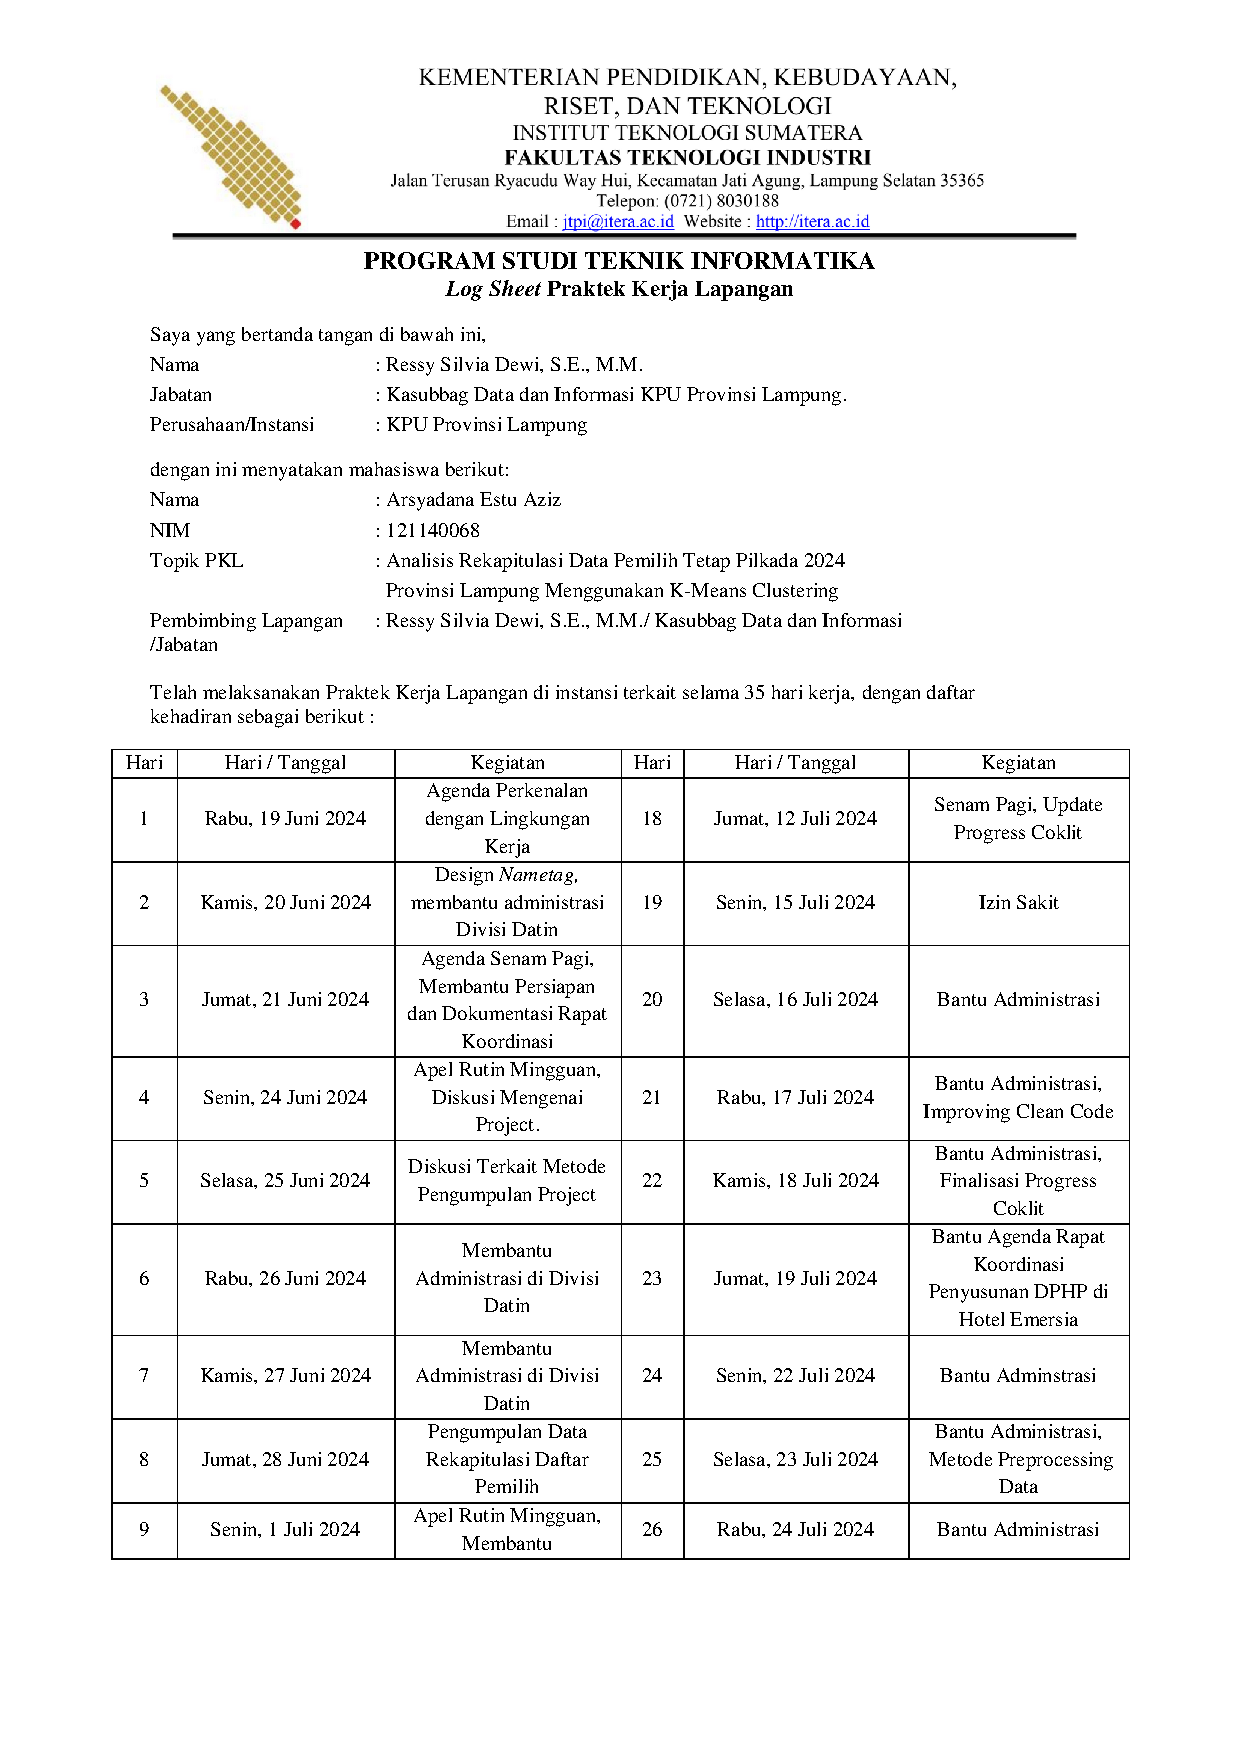
\includepdf[pages=-,scale=.8,pagecommand={\centering \section*{Lampiran Logsheet}\label{}},linktodoc=true]{document/logsheet-kp.pdf}

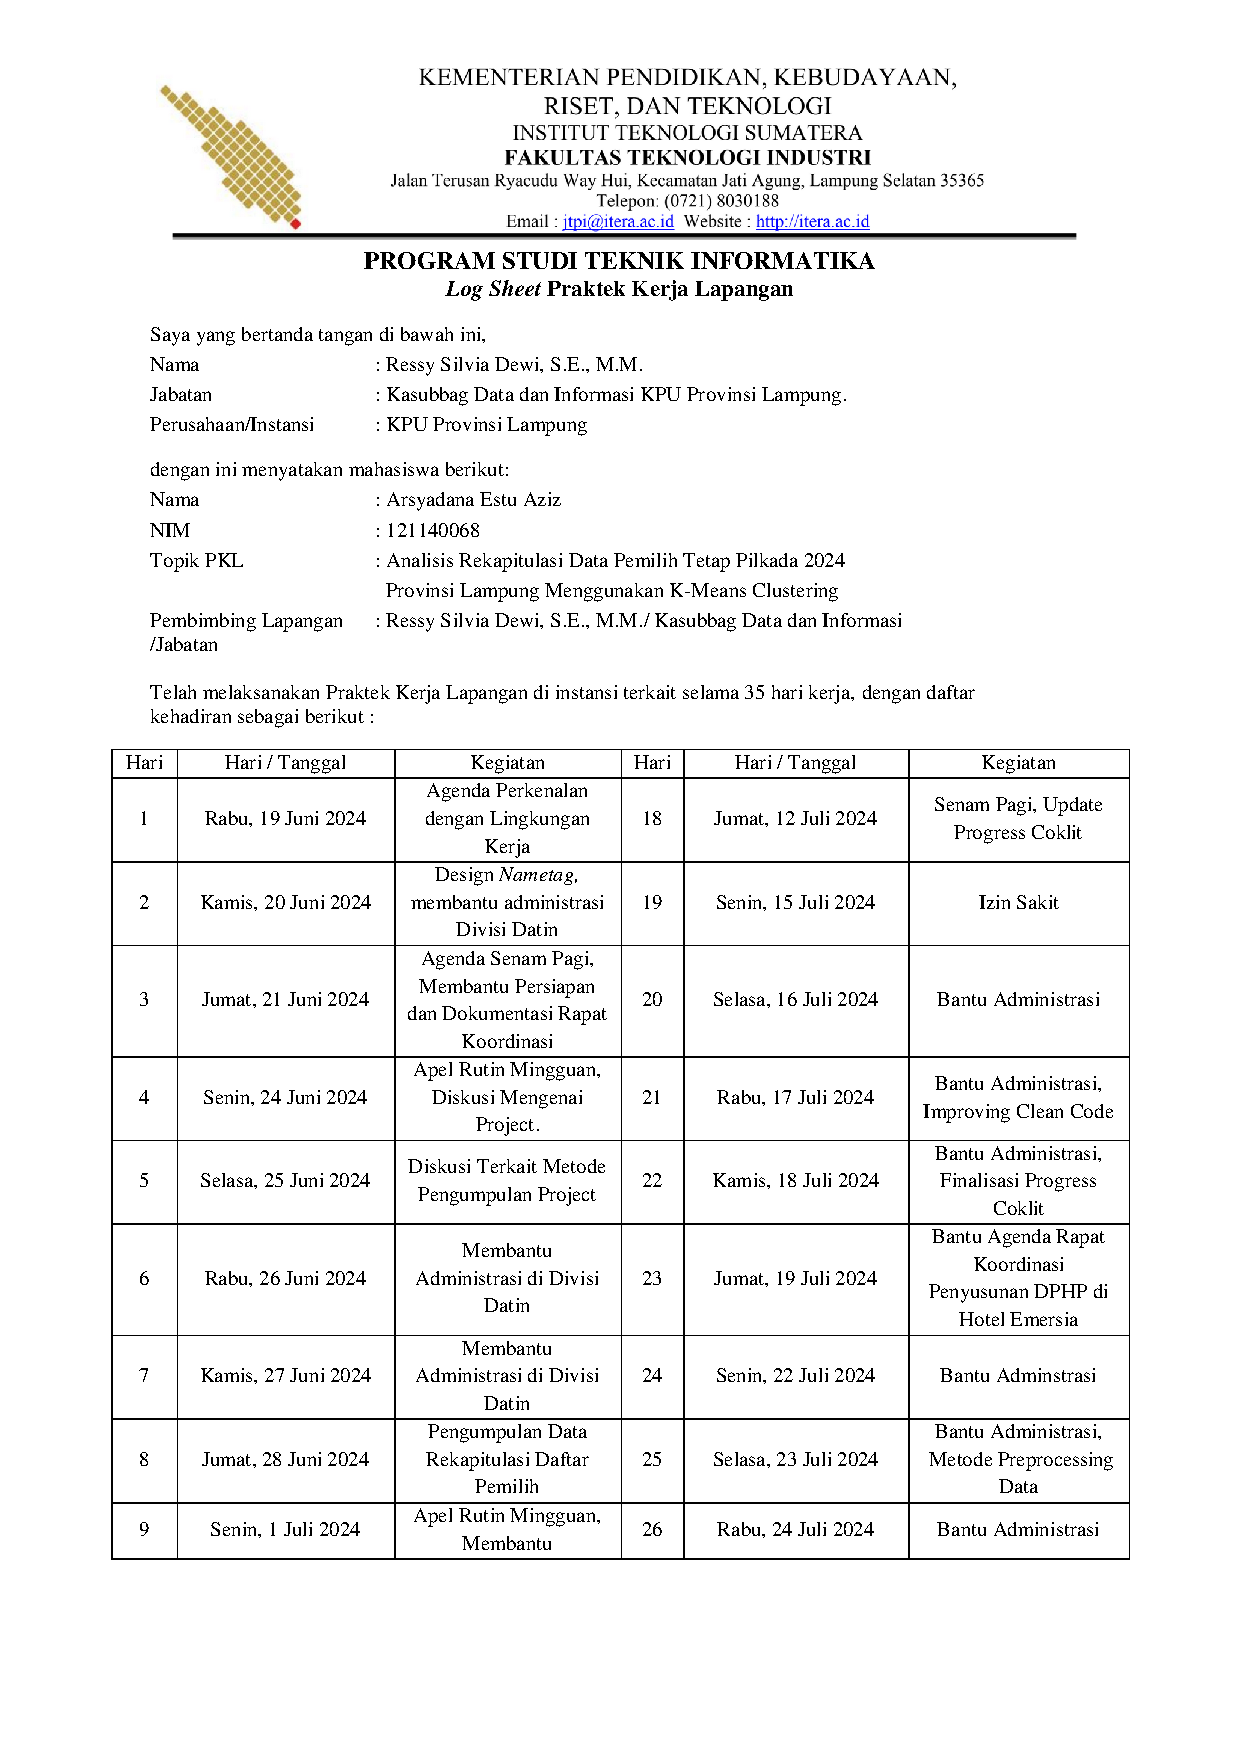
\includepdf[pages=1,scale=.8,pagecommand={\centering \section*{Lampiran B. Log Sheet} \addcontentsline{toc}{section}{Lampiran B. Log Sheet} \label{pdf:myfile}},linktodoc=true]{document/logsheet-kp.pdf}
\includepdf[pages=2-,scale=.8,pagecommand={},linktodoc=true]{document/logsheet-kp.pdf}


